6\section{\label{sec:scale}Scaling Analysis}
The Gung Ho dynamical core uses an unstructured mesh to avoid a
singular pole which ultimately inhibits the scaling of the
UM. Examining the scaling behaviour of the model to see if it
performs sufficiently well is therefore important. To test the scaling a series
of model runs was performed. The version of the LFRic repository trunk
was $17483$. The code was compiled on the XCS with the Intel 17
compiler, at production level which is \verb+-O3+. The baroclinic wave
test was run on a $C576$ mesh. This roughly corresponds to a $17$km
horizontal resolution. The model was run with a $30$km lid and with
$30$ levels.  The time-step used was $180$
seconds and the benchmarks were run for $100$ time-steps. The code was
profiled using the CrayPAT tool in sampling mode. 

\begin{figure}
\centering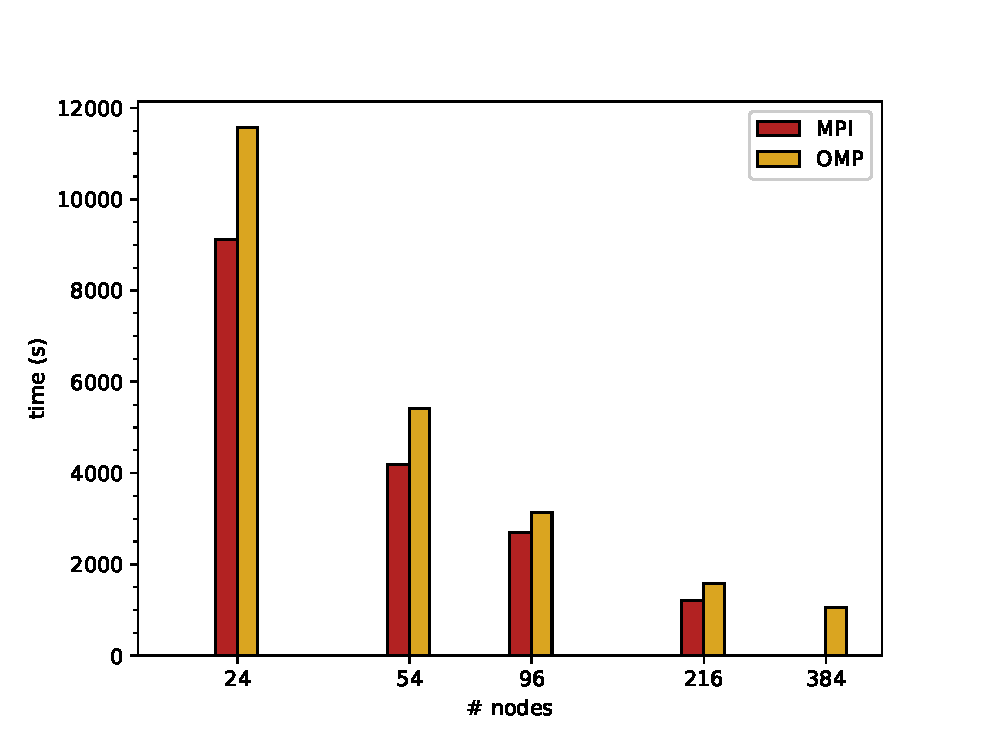
\includegraphics[width=1.0\linewidth]{figs/wc-scale.eps}
\caption{\label{fig:wc_scale}Wall-clock time strong scaling of the 
  Baroclinic wave test. In red, labelled MPI is an MPI only
  version. In yellow, labelled OMP is the hybrid MPI+OpenMP version.}
\end{figure} 

Shown in figure~\ref{fig:wc_scale} is the strong scaling of the whole
model up to $384$ nodes. The MPI only version ran with $36$ MPI ranks
per node. The hybrid version ran with $6$ MPI ranks per node and $6$
OpenMP threads per MPI rank. The MPI only version on $384$ nodes
crashed during the partitioning phase with an Out Of Memory (OOM)
error. The global mesh is read in by every MPI rank and then
partitioned. This can cause memory problems for large meshes on larger
node counts. This can be solved by a single rank per node reading in
the mesh and broadcasting the partition\footnote{This has yet to be implemented.}. The $24$ node hybrid job ran
out of time after 3 hours at $93$ time-steps, so the run time has been
estimated from the log data. This data is also shown in
table~\ref{tab:scale-data}.

\begin{table}
\centering
\caption{\label{tab:scale-data}Wall-clock time of execution of the whole code (WC), User
  code (U), Halo Exchange (HE) and Global Sum (GS) in seconds. Also
  shown is the Local Volume per MPI ranks (LV) and the Halo Size (HS)
  measured in number of horizontal cells.}
\begin{tabular}{r|rrrr|cr}
N & WC & U & HE & GS & LV & HS  \\
    & \multicolumn{4}{c|}{time (s)} & \multicolumn{2}{c}{cells} \\ \hline\hline
     &  \multicolumn{4}{c|}{MPI}& \\
$24$  & $9126$ & $4107$ & $788$ & $502$ & $48\times 48$ & $196$ \\
$54$  & $4196$ & $3139$ & $411$ & $470$ & $32\times 32$ & $132$ \\ 
$96$  & $2693$ & $1508$ & $380$ & $679$ & $24\times 32$ & $100$ \\ 
$216$ & $1202$ & $566$  & $302$ & $174$ & $16\times 16$ & $68$  \\ 
$384$ & $--$   & $--$   & $--$  & $--$  & $12\times 12$ & $54$ \\\hline
  & \multicolumn{4}{c|}{Hybrid} & \\
$24$ &$11566$ & $--$    & $--$  & $--$ & $96\times 144$ & $484$ \\
$54$ & $5410$  & $2732$ & $1282$ & $887$ & $64\times 96$ & $324$ \\
$96$ &$3140$  & $1332$ & $895$ & $562$ & $48\times 72$ & $244$ \\
$216$ &$1585$  & $468$ & $485$ & $384$ & $32\times 48$ & $164$ \\
$384$ &$1059$  & $222$ & $310$ & $322$ & $24\times 32$ & $124$
  \\\hline
  & \multicolumn{4}{c|}{MPI 4, OMP 9} & \\ 
$96$ & $4183$ & $1338$ & $1296$ & $1104$ & $72\times 72$ & $292$ \\ \hline
\end{tabular}
\end{table}

The model shows good scaling for both the MPI and hybrid programming
models. The parallel efficiency is reasonable, the $216$ node job uses
$9\times $ the resources of the $24$ node job and both the MPI and
hybrid version run more than $7\times $ faster. The hybrid code for the
$384$ node job which has $16\times $ the resource of the $24$ node
job, runs approximately $11 \times$ faster.

Compared to the scaling runs performed with the {\em Fallow Deer} (FD)
release of LFRic and reported in~\cite{LFRic} there is an apparent
change in the OpenMP behaviour. The FD scaling shows the hybrid version of
the code is faster than the MPI version, whereas the opposite is now
true for the data displayed here. It is unclear why this might be
so. The science problem and parallel code are broadly the same. The
major change is to the solver algorithm which uses the new solver
API. However, it is far from obvious why this would change the
behaviour.

The jobs have been profiled with CrayPAT and the data is shown in
table~\ref{tab:scale-data}. CrayPAT groups the data according certain
categories. User code (labelled ``U'') in the table is the LFRic
code, in this case kernels such as the various matrix-vector
routines. The Halo Exchanges (labelled ``HE'') appear in the external library
category as YAXT is compiled as a library, in this case without the
CrayPAT profiling, so it is unable to see that this ultimately calls
MPI. The Global Sums (labelled ``GS'') appear under {\em MPI} as the
global summation calls are in the LFRic infrastructure code.

The strong scaling of the user code is shown in
figure~\ref{fig:U_scale}\footnote{There is no hybrid data for 24 nodes
  as the model didn't run to completion so no profile was generated.}.
Both the MPI only and hybrid code show excellent scaling - the
communication costs are represented in other categories. For MPI
only, comparing the $24$ node to the $216$ node jobs, the User code
runs nearly $9\times$ faster for $9$ times the resource. The hybrid
version fares even better, showing super-linear scaling. Comparing the
$54$ node job to the $384$ node job, the user code runs more than
$12\times$ faster for $7.11\times$ the resource. This may well be due
to caching effects, once the local volume becomes small enough to fit
into cache.


\begin{figure}[ht!]
\centering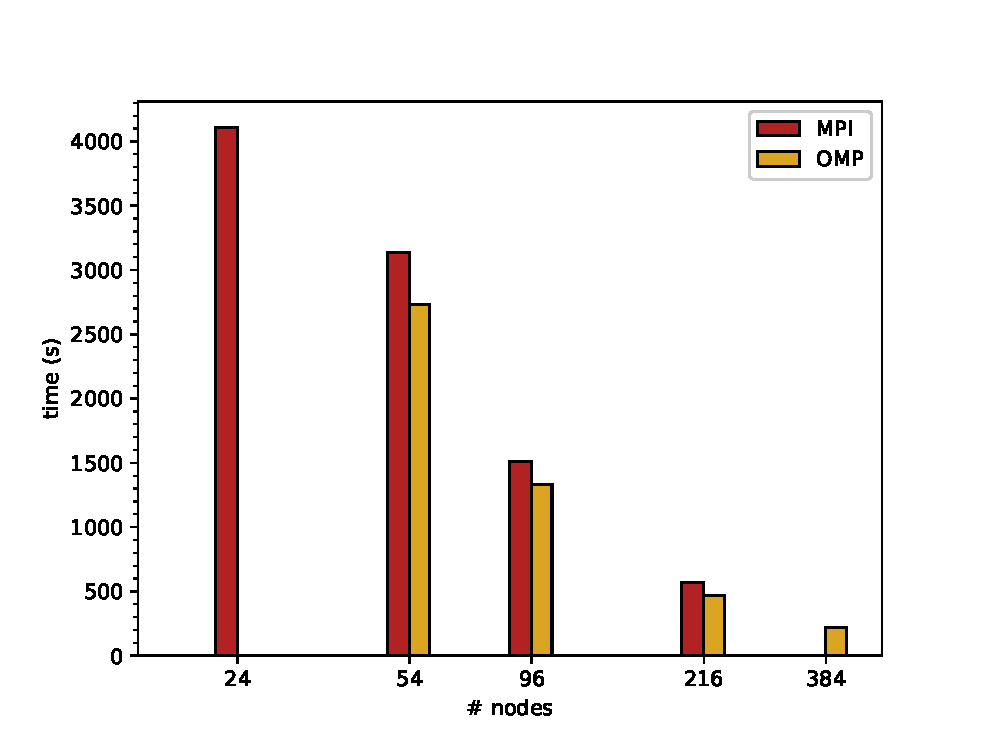
\includegraphics[width=1.0\linewidth]{figs/U-scale.eps}
\caption{\label{fig:U_scale}Wall-clock time strong scaling of the 
  User code from Baroclinic wave test.}
\end{figure} 

Shown in figure~\ref{fig:comms_scale} and Table~\ref{tab:scale-data}
is the strong scaling of the communication components as measured by
the CrayPAT tool. The halo exchanges for hybrid version of the code
takes significantly longer than the MPI only version. The time
difference accounts for the hybrid version being slower than MPI only.
The count of the number of halo exchanges (performed internally by
LFRic) is almost the same for the MPI and hybrid versions. The
difference is a few hundred out of a total of $1.3$ million. The are
not exactly the same because the global sum is not reproducible across
different partitions, so the evolution is slightly different. However,
after $100$ time-steps and many thousands of solver iterations, the
conservative fields are still the same to many orders of magnitude.

\begin{figure}[ht!]
\centering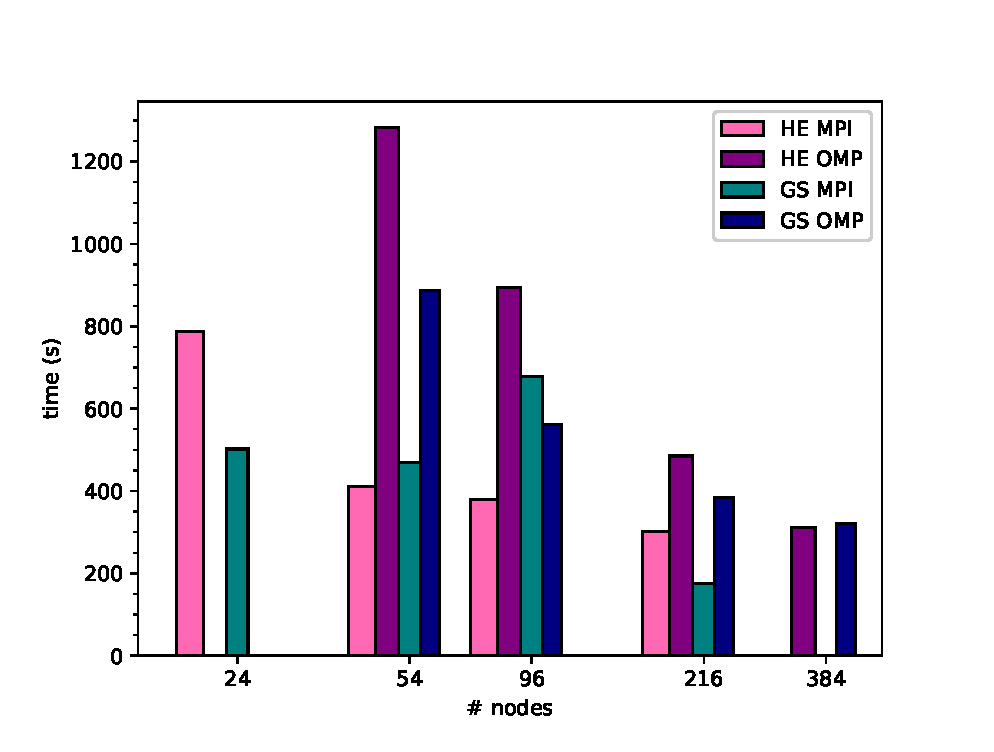
\includegraphics[width=1.0\linewidth]{figs/comms-scale.eps}
\caption{\label{fig:comms_scale}Wall-clock time strong scaling of the 
  communications costs of the Baroclinic wave test. HE denotes Halo
  Exchange and GS the Global Sum.}
\end{figure} 

The size of the halos is shown in Table~\ref{tab:scale-data}. The 
halos for the hybrid version are bigger than the MPI only version, as 
there are fewer MPI ranks, but there are less messages to send. As the 
hybrid version is running with six threads, it has six times less the 
number of messages. The hybrid version has fewer, but bigger MPI 
messages and moreover, will have less total data to send. It is not 
obvious why it should be so much slower. 

The global sums don't show a clear trend in the case of MPI only and
they appear to get faster with more nodes for the hybrid version. This
is perhaps counter intuitive as the global sum is latency bound and
should increase with the number of nodes. However, the aries network
employs adaptive routing so that the path taken for communication
depends on what other network traffic is occurring at the same
time. This results in the best use of the total network, but for an
individual application the communication cost may not be optimal and
worse, not deterministic.

To try and remove the effect of this variability, a Cray environment
variable \verb+GNI_BLAS+ was set to $2$ and the $96$ node jobs re-run.
Whist there was a difference between the run-times, the less adaptive
version was not consistently faster, nor did it change the balance
significantly. It should be noted that the communication cost
node imbalance for the hybrid mode is significantly higher than for MPI
only. The imbalance (defined as the variation across MPI ranks) is
around $15\%$ of the halo exchange cost, which rises to $30\%$ of a
much larger number for the hybrid version. For the global sum, again
there is a much larger variation for the hybrid version even if the total time spent in
global sums is reduced compared to MPI only. Changing the Cray
environment variable settings does not materially change this view. 

Also shown in Table~\ref{tab:scale-data} is the CrayPAT profile data
for a $96$ node job run with $4$ MPI ranks per node and $9$ OpenMP
threads per MPI rank. This has a square domain decomposition like the
MPI only versions. This runs considerably slower than both the $6$
thread and MPI only version. The OpenMP synchronisation cost barely
shows in the profile at $1\%$ of run-time. The user code portion runs
in roughly the same time as the $6$ thread version, which is faster
than MPI only. However, the communication costs are much higher. Both
Halo Exchange and Global Sum take much longer and have a high degree
of imbalance, at around $30\%$ each. The number of Halo Exchanges is
around 1.3 million, the same as MPI and $6$ thread versions.  It is
reasonable to believe that at least some of this increase in cost is
due to network variablility. This could be examined by running in
large exclusive reservations or with a statistical analysis of a large
number of runs. Both of these are expensive in terms of resource use and
probably unjustifiable given pressure on resources for science rather
than performance evaluation.

It is also not obvious why the hybrid version should now be slower
than MPI when the opposite was true in the FD release. In this data
the time-step is longer at $180$s and moreover, the FD data was not
profiled using CrayPAT, but the time for $50$ time-steps can be calculated
from the logs. Shown in table~\ref{fig:fd_comp} is a comparison of
trunk at r17483 and the FD release. Clearly the hybrid version is now
much slower. The trunk versions uses the new solver API, so the solver
is a different algorithm but it is not doing a significantly different
number of halo exchanges. Neither the YAXT library performing the halo
exchanges nor the generated PSy layer code are any different, {\em
  i.e.} halo exchanges called outside OpenMP regions, which call halo
exchange on fields, which call YAXT. However,
given the large cost of halo exchange for the hybrid version of trunk
it is not unreasonable to surmise that this is the difference between
FD and trunk.

\begin{table}
\centering
\caption{\label{fig:fd_comp}Comparison of $50$ time-steps for the model on $96$ nodes
  with a $75$s time-step.}
\begin{tabular}{ccc}
Run & time(s) & HE count \\\hline
FD MPI & $714$ & $--$ \\
FD OMP & $606$ & $697381$ \\
Trunk OMP & $999$ & $755657$  
\end{tabular}
\end{table}

In summary the LFRic model shows very good scaling behaviour for both
MPI only and hybrid versions. The halo exchanges for the hybrid
version are now performing worse than MPI only, and worse than in the
fallow deer release. The reasons for this are unclear and whilst the
variability of the communication cost due to the adaptability of the
Aries network has some role to play, it is not obvious that this is
the reason for the degradation of communication performance. Reducing
the communication costs are a target for improving the scalability of
the model. In the next sections, approaches to reducing the global
and local communication costs are described.